% This is "sig-alternate.tex" V2.0 May 2012
% This file should be compiled with V2.5 of "sig-alternate.cls" May 2012
%
% This example file demonstrates the use of the 'sig-alternate.cls'
% V2.5 LaTeX2e document class file. It is for those submitting
% articles to ACM Conference Proceedings WHO DO NOT WISH TO
% STRICTLY ADHERE TO THE SIGS (PUBS-BOARD-ENDORSED) STYLE.
% The 'sig-alternate.cls' file will produce a similar-looking,
% albeit, 'tighter' paper resulting in, invariably, fewer pages.
%
% ----------------------------------------------------------------------------------------------------------------
% This .tex file (and associated .cls V2.5) produces:
%       1) The Permission Statement
%       2) The Conference (location) Info information
%       3) The Copyright Line with ACM data
%       4) NO page numbers
%
% as against the acm_proc_article-sp.cls file which
% DOES NOT produce 1) thru' 3) above.
%
% Using 'sig-alternate.cls' you have control, however, from within
% the source .tex file, over both the CopyrightYear
% (defaulted to 200X) and the ACM Copyright Data
% (defaulted to X-XXXXX-XX-X/XX/XX).
% e.g.
% \CopyrightYear{2007} will cause 2007 to appear in the copyright line.
% \crdata{0-12345-67-8/90/12} will cause 0-12345-67-8/90/12 to appear in the copyright line.
%
% ---------------------------------------------------------------------------------------------------------------
% This .tex source is an example which *does* use
% the .bib file (from which the .bbl file % is produced).
% REMEMBER HOWEVER: After having produced the .bbl file,
% and prior to final submission, you *NEED* to 'insert'
% your .bbl file into your source .tex file so as to provide
% ONE 'self-contained' source file.
%
% ================= IF YOU HAVE QUESTIONS =======================
% Questions regarding the SIGS styles, SIGS policies and
% procedures, Conferences etc. should be sent to
% Adrienne Griscti (griscti@acm.org)
%
% Technical questions _only_ to
% Gerald Murray (murray@hq.acm.org)
% ===============================================================
%
% For tracking purposes - this is V2.0 - May 2012

\documentclass{sig-alternate}
\usepackage{algorithm}
\usepackage[noend]{algpseudocode}
\usepackage{mathtools}
\begin{document}
%
% --- Author Metadata here ---
\conferenceinfo{WOODSTOCK}{'97 El Paso, Texas USA}
%\CopyrightYear{2007} % Allows default copyright year (20XX) to be over-ridden - IF NEED BE.
%\crdata{0-12345-67-8/90/01}  % Allows default copyright data (0-89791-88-6/97/05) to be over-ridden - IF NEED BE.
% --- End of Author Metadata ---

\title{NSGA 2 For City Planning}
\subtitle{[Special Project Report]}
%
% You need the command \numberofauthors to handle the 'placement
% and alignment' of the authors beneath the title.
%
% For aesthetic reasons, we recommend 'three authors at a time'
% i.e. three 'name/affiliation blocks' be placed beneath the title.
%
% NOTE: You are NOT restricted in how many 'rows' of
% "name/affiliations" may appear. We just ask that you restrict
% the number of 'columns' to three.
%
% Because of the available 'opening page real-estate'
% we ask you to refrain from putting more than six authors
% (two rows with three columns) beneath the article title.
% More than six makes the first-page appear very cluttered indeed.
%
% Use the \alignauthor commands to handle the names
% and affiliations for an 'aesthetic maximum' of six authors.
% Add names, affiliations, addresses for
% the seventh etc. author(s) as the argument for the
% \additionalauthors command.
% These 'additional authors' will be output/set for you
% without further effort on your part as the last section in
% the body of your article BEFORE References or any Appendices.

\numberofauthors{3} %  in this sample file, there are a *total*
% of EIGHT authors. SIX appear on the 'first-page' (for formatting
% reasons) and the remaining two appear in the \additionalauthors section.
%
\author{
% You can go ahead and credit any number of authors here,
% e.g. one 'row of three' or two rows (consisting of one row of three
% and a second row of one, two or three).
%
% The command \alignauthor (no curly braces needed) should
% precede each author name, affiliation/snail-mail address and
% e-mail address. Additionally, tag each line of
% affiliation/address with \affaddr, and tag the
% e-mail address with \email.
%
% 1st. author
\alignauthor
Dr. Bistra Dilkina\\
%	\affaddr{Institute for Clarity in Documentation}\\
%	\affaddr{1932 Wallamaloo Lane}\\
%	\affaddr{Wallamaloo, New Zealand}\\
%	\email{agupta375@gatech.edu}
% 2nd. author
\alignauthor
Parminder Bhatia\\
%	\affaddr{Institute for Clarity in Documentation}\\
%	\affaddr{P.O. Box 1212}\\
%	\affaddr{Dublin, Ohio 43017-6221}\\
	\email{parminderb@gatech.edu}
% 3rd. author
}
% There's nothing stopping you putting the seventh, eighth, etc.
% author on the opening page (as the 'third row') but we ask,
% for aesthetic reasons that you place these 'additional authors'
% in the \additional authors block, viz.
\additionalauthors{Additional authors: John Smith (The Th{\o}rv{\"a}ld Group,
email: {\texttt{jsmith@affiliation.org}}) and Julius P.~Kumquat
(The Kumquat Consortium, email: {\texttt{jpkumquat@consortium.net}}).}
\date{30 July 1999}
% Just remember to make sure that the TOTAL number of authors
% is the number that will appear on the first page PLUS the
% number that will appear in the \additionalauthors section.

\maketitle


\terms{Theory}

\keywords{ACM proceedings, \LaTeX, text tagging}

\section{Introduction}
Spatial Optimization is one of the most important problem in computational sustainability today. For the purpose of understanding ,we can consider that if we are given a raster matrix (M*N), spatial optimization can be described as allocation of land types (Commercial, Residential, Green, Industrial,  Recreational) to each of the cells /land mass under given constraints (money, contiguity, future expansion etc.).  Spatial Optimization is challenging because it involves lots of dependencies, variables, objectives and input parameters. And as these features increase the problems becomes more complex and it grows exponentially. Solving such a massive problem manually is out of question. We need computational tools to better understand all the aspects of such a gigantic problem.
Comprehensive sustainability in urban planning can be termed as a long-term balance between economic development, environmental protection, efficient resource use, and social equity


Spatial Optimization can also be looked as a demand-constraint problem, where objective is to allocate land type of given land masses keeping in mind the various constraints. The abstract concept of constraints on which  desired constraints and objectives are build are :-
Continuity
Compactness
Compatibility

\graphicspath{ {images/} }
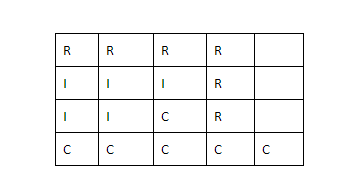
\includegraphics{raster}

\subsubsection*{Continuity} - Continuity can be defined as as the degree to which a specific use has been allocated to land in an unbroken fashion. It basically refers to the connected component of the same type. Here, in the figure we can see that C has very high contiguity.

\subsubsection*{Compactness} - We define compactness as an allocation of a given land use to sites that are in direct proximity of each other, resulting in circular patches. In the figure above, we can see that land type I has maximum compactness.

\subsubsection*{Compatibility} - Compatibility  as the word suggests refers to how compatible a given land use type is with his neighbour(other land type) . We would prefer to have green areas close to residential as compared to having industry close to residential, thus compatibility index of the former will be higher.\\[.25cm]

\section{Problem Definition}

In a land usage optimization problem, finite amount of resources (commercial, industrial, residential area etc.) are allocated effectively to a specific land mass under given constraints (money, contiguity, future expansion etc.). In fact it has been depicted that inefficient resource use leads to high traffic congestion and other sustainability issues (Newman et al.). Therefore, it is important to carefully design land use allocation models. Since, land use allocation is a resource allocation problem for a given space, therefore many times it is considered as a spatial optimization problem. \\
This problem was first addressed by Schlager et al. as a Linear Programming model in 1965 and it was mostly constrained to single objective optimization. Since this problem is much more complex and involves a lot more objectives, therefore multi-objective approach was adopted by other researchers (mentioned in following section).  Many researchers however constrained themselves by still continuing with Linear Programming approach and by assigning different weights to different objectives and performing linear combinations to attain the solution.It is a major issue for planners to numerically quantify the relative weights of each of the defined objective. Moreover, non-convex optimal solutions cannot be obtained by minimizing linear combinations of objectives.


Due to the multifaceted nature of land-use allocation, spatial optimization modelling should aim at finding a set of high-performing alternatives instead of just one solution (Bankes 1993, Church 1999, Harris 2001) and allow the stakeholders to choose from a number of scenarios that are both good and different from each other, since not every planning objective of interest may be introduced into the
model in the form of mathematical formulation (Chang et al. 1983, Brill et al. 1990). The decision-makers should be provided with alternatives that allow for consideration of other—less defined—planning goals, or recognition of overlooked issues and innovative solutions (Chang et al. 1983). Consequently, the generated alternatives should be treated not as ultimate solutions but as propositions for further analysis by stakeholders.

\section{Related Work}
In this section we provide a basic overview of the existing models and papers, which we provides the background of our current work. Details on these papers can be found in the last section of the paper. \\
\subsection{Sustainable Multi-objective Land Use Allocation (SMOLA)}  Zelinska had conceptualized this approach wherein MOLA model is improved by incorporating the Generative Hop Skip Jumps (HSJ) techniques on top of the MOLA model. The land mass is divided into homogenous cells and further optimization and computations are performed to obtain three objectives: compactness, compatibility and contiguous residential patterns. Multi-objective land-use allocation is adopted to minimize the incompatibility with the adjacent land uses (cells). Sustainable land-use allocation is defined as a normative modelling methodology, which focuses on evaluating current land-use patterns and introduces the changes to increase the compatibility with the adjacent cells, compactness, infill- development and political defensible redevelopment. They have also tried linking the optimization problem with GIS. Moreover, this model leaves many questions open-ended such as developing heuristics on top of it, more dynamic setting etc., which need further research. \\

\subsection{Non-dominated Sorting Genetic Algorithm-II (NSGA-II)} Pertaining to two goals in a multi-objective problem (i.e. Convergence to Pareto-optimal and diversity), NSGA-II has proved to be very effective approach since it provides both of these objectives. Furthermore, it considers the multi-objective nature of the problem it tries to reduce the complexity of the problem, by using non-dominated sorting and crowding distance for computational purposes.\\

\subsection{ NSGA-II Multi Objective Land Usage  ( NSGA-II -MOLU )} In an land use optimization problem, as the features and spatial attributes increase the problem grows exponentially too. Recently, Cao and Roberts et al. have used the spatial optimization problem using this approach (NSGA-II-MOLU). In this method, population is sorted at different fronts using the non-dominated ranking method with a particular book-keeping strategy which improves the computational complexity of the problem. When solving a problem using GA, chromosomes can be defined in two ways: fixed length representation (land uses as genes, sensitive to number of parcels) and variable length representation (sensitive to land types). Incorporating these features diversity can be maintained. However, they have considered only three spatial objectives: minimizing conversion costs, maximizing accessibility and maximizing compatibility, but this model promises efficiency over generality. \\

\section{Formal Model}

In order to define and elaborate on our model, we first provide a set of inputs and variables which will be used in our model .\\
\paragraph{Inputs\\}
\begin{itemize}
\item  \textbf{Landuse }: Landuse specifies the type of land allocation to that particular area.
\item Area : $A_j$ is the area of the parcel j.
\item $Y_j$ is the initial land use type of parcel $j \in V$
\item V : Refers to all the parcels /cells
\item U : Refers to set of parcels that are undeveloped ,i.e.
$ Y_{i} = 0$ , where  $Y_{i}$ refers to the land use type. 
\item $N_j$ : Neighbours of parcel $j \in V$    
\item \textbf{Attractiveness} : We define $a_j$  as the measure of attractiveness of an undeveloped location for development. 
$ a \in (0,1)$
\item Compatibility : $\partial_{kk'}$ refers to compatibility of landuse type k with k', where k,k' $\in {0,..N}$
\item : Closest Neighbour -  $dist_j$ refers to distance from j to closest developed neighbour cell.
\item $\vartheta_{kk'} $ - Refers to the conversion cost from  type k to k'
\item $s_j$ : Number of initially developed neighbours of j , $$ s_j = \sum_{i \in N_j: Y_i \neq 0} 1$$
\item $rd_j$ : road distance to the closest road from cell  j
\item roadDist(dis,k) : It is the penalty for distance from road for type k

\end{itemize}

\paragraph{Variables\\}
\begin{itemize}
\item  To refer to particular area we will use the notation $X_{ik}$, where land/pixel i is assigned a landuse type k. LandUse Types can take values from 0 to N, where N is the number of landuse types. We will always refer to 0 as the undeveloped land type and others would be enumerated depending upon the number of land types available.\\
Every parcel follows the following assignment constraint.

\subsubsection*{Assignment Constraint}
$$\sum_{k=0}^N A_j X_{jk} =1$$
This equation basically tells us that, every parcel,must have one and only one assignment of a landuse type .
\end{itemize}
\paragraph{Potential Objectives and Constraints}
\begin{itemize}
\item
\subsubsection*{Minimize Undeveloped Land}

We define $ a_{j},$ as the attractiveness of an undeveloped location for development. Higher value indicates higher attractiveness towards development.  Thus, we can have low value for undeveloped open places. and minimize the following

 $$
 min\sum_{j \in U} (1-a_j) \sum_{k=1}^N X_{jk}
 $$
Consider values $a_j$  for all cells that encode attractiveness for development for undeveloped cells. Idea is to set $a_j$ very low for cells in open space. Add objective to minimise summation of (1-$a_j$) for all undeveloped cells that are developed. 

\item 
\subsubsection*{ Compatibility(Generic  version of Contiguity)}
All earlier papers have tried to make use of compatibility by keeping static locations , where they compare compatibility of new allocation with respect to static initial allocation.\\[.15cm]
$
max \sum_{j \in U} \sum_{i \in N_j}(\sum_{k=0}^{N}\partial_{kk'} X_{jk} X_{ik'}) 
$ 
$$+ max (\sum_{j \in V} \sum_{i \in N_j}(\sum_{k=0}^{N}\partial_{kk'} X_{jk} X_{ik'}))
$$
 This basically means , that we assume neighbors to be same(static across the selection) 

We would like to maximize compatibility of a cell wrt its neighbours.
$$
max \sum_{j \in V}  \sum_{i \in N_j}(\sum_{k=0}^{N}\sum_{k'=0}^{N}\partial_{kk'} X_{jk} X_{ik'})
 $$
Here $N_j $ are neighbours of j. Thus we want development such that compatibility is maximised. Simple equivalent of this would be to have $\partial_{kk'} = 1 $ if  $k =k'$ else $0$. Thus, contiguity can be seen as a special case of compatibility ,where we basically look to maximize contiguous areas with  a particular LandType.

\item
\subsubsection*{Demand Constraint  }
 Total area for each type should remain in the upper and lower bound of the limits provided.
$$ L_k < \sum_{j \in V} \sum_{k=0}^N X_{jk} < U_k $$
\item

\subsubsection*{Minimize land conversion }
Minimize land conversion -- Conversion cost refers to the cost associated with changing the landuse type of parcel from one type to another.
$$
 min\sum_{j \in V}  \sum_{k=1}^N (\vartheta_{Y_{j}k}) X_{jk}
 $$
In the simple version, we can keep $\vartheta_{Y_{j}k} =  1$ for all k where $k \neq Y_{j},0$
\item
\subsubsection*{ New Development}
Next objective is to keep new developments close to existing developments
 $$
 min\sum_{j \in U}(dist_j) \sum_{k=1}^N X_{jk}
 $$


\item
\subsubsection*{Compact Development -- Infill development}
All earlier papers have tried to make use by keeping static locations , where they compare compact development of new allocation with respect to static initial allocation.
Idea is that if j is developed then atleast b of his neighbours should be developed.
$$
s_j +\sum_{i \in N_j, Y_{i} =0 } \sum_{k"=0}^N X_{ik"} >= b \sum_{k=0}^N X_{jk}
 $$
\item
\subsubsection*{Accesibility  }
Idea is that particular development should be close to road for accessiility purposes. We are keeping it simple assuming only a single type of road, which can be extended further.
 $$
 min\sum_{j \in V} \sum_{k=0}^N roadDist(rd_j,k)X_{jk}
 $$



\end{itemize}

\section{Approach}

\subsection{Genetic Algorithms }

GAs are one of several strategies including EA and Genetic Programming that have come to be known as Evolutionary Strategies (Beyer 2001). Evolutionary Strategies are members of a class of optimizers referred to as heuristic methods. GAs have been shown to perform well in a variety of engineering optimization applications including those with single, multi-modal, and multiple objective functions (Zitzler et al. 2001; Quagliarella et al. 1998; Dasgupta and Michalewicz 1997; Mazumder and Rudnick 1999; Rahmat-Samii and Michielssen 1999). In fact, as Zitzler et al. (2001) illustrate, these types of approaches form the relatively new field of EMO.\\
In a Simple GA (SGA), initial solutions are coded as a randomly generated set of strings or real numbers and better solutions are iteratively evolved using stochastic methods that include selection, crossover, and mutation operators (Mitchell 1996). The algorithm starts by randomly generating a fixed number of initial chromosomes (usually binary strings) that code potential problem solutions. The main part of the algorithm is an iterative process that evaluates all solutions in the current generation with a fitness function(s). The best performing solutions are selected to be parents. Crossover and mutation operators are applied to these parent chromosomes to produce a pair of offspring solution chromosomes. In other words, combining the best performing solutions from a population of solutions allows better solutions to evolve. The iterative process is continued until a prescribed maximum number of generations (iterations) has been completed. Note that the maximum number of generations is a user-specified parameter which most often is dictated by available computer resources.\\
\subsection{NSGA 2}
A modification to the SGA, the Non-dominated Sorting Genetic Algorithm-II (NSGA-II), is used in this paper. The NSGA-II allows the GA methodology to be applied to multi-objective problems. The NSGA-II is based on the idea of Pareto optimality, but it extends this notion by considering an ordering or ranking of solutions based on the non-dominance of solutions on the Pareto front and introduces elitism by retaining the last generation as part of the pool for new selections. \\[.25cm]

Following are the concepts used in our implementation pertaining to NSGA\\[.10cm]
\textbf{Generator}- Initially , we generate a sample of dataset. They are generated based on initial configuration and set of allowed changes for some of the parcels. \\[.15cm]
\textbf{Evaluator }- In the evaluator , we basically evaluate the  given candidates based on the objective functions and sign score to each candidate.\\
Based on these scores next generation candidates are selected from the given candidates . \\ [.15cm]
\textbf{Mutation }- In the mutation and initial generation for NSGA, we have made sure that each parcel gets value from the allowed lands type for the particular parcel, which makes sure that we don't generate any infeasible solution.\\[.35cm]


\subsection{Supported Objectives}

With view to validate the Objectives and Constraints defined above, we have implemented the above objectives to observe the impact  of these objectives and constraints.\\[.25cm]

We have implemented the following Objectives:

\paragraph*{Contiguity/Compatibility}

We implemented the special version of contiguity for this objective, where we give weight of 1 to $\lambda_{ij}$ if i and j are same and 0 otherwise.
We  take the continuity objective as a dynamic constraint, where we take the fitness score wrt to current assignment of the candidate. We evaluated the contiguity by checking for the neighbors which have same assignment of LandUse type as the LandUse type of a particular parcel. We evaluated the neighbors Landuse type based  on the dynamic / current assignment of the candidate.

\paragraph*{Demand Constraints/Limits}

We implemented the Limits constraint as an  objective. We try to minimize this objective. High penalty is given incase the objective does not lie the limits and max negative value is given for land type in the middle of max-min allowed for the above lands type. We want all land use type to be within the min-max limit allocated for the landuse type. We have taken couple of approaches in this. Simple one is to simple give 0 weight when within the limit and apply penalty equal to the extent with which lands is above or below the limit( linear) .Second approach is that instead of simply keeping 0 we made a linear triangle with in the limit which was maximum at center of max-min and give higher penalty when out of range. Note that using this approach gives us a higher bound and more penalty incase of getting out of limits. 

\paragraph*{Attractive}

We implemented the Attractiveness  objective, where we try to minimize this objective. This objective basically suggests that more the attractive of unused land type higher are the chances of it getting developed. Attractiveness(a) is defined as willingness of a cell/parcel towards development. We evaluate (1-a) , thus this value will be initially 0 and increase as we change undeveloped cells to developed. Our objective is to minimize this value, thus cells having high attractiveness value will be developed in preference to others.

\paragraph*{Conversion}

We implemented the Conversion  objective, where we try to minimize this objective. Minimize land conversion -- Conversion cost refers to the cost associated with changing the Land use type of parcel from one type to another. Attractiveness is basically a special case for conversion, where in addition to the values for undeveloped parcels, $a_i$ is 1 for all the developed parcels.\\



\section{Synthetic Dataset}

\subsection{Dataset}
In order to validate our objectives, we first analysed our algorithm on a small dataset represented by 10X10  , as shown in the figure.
\begin{figure}[h]
\begin{center}
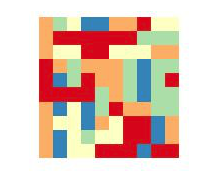
\includegraphics[width=3.in]{orig.png}
\caption{Synthetic Dataset used for initial evaluation}
\end{center}
\end{figure}

In this raster we have 5 types of the LandUse types - Undeveloped, Green, Residential,Commercial and Industrial. Land Type area has been provided in the table below.\\
Here the red region corresponds to undeveloped region.\\
\begin{figure}[h]
\begin{center}
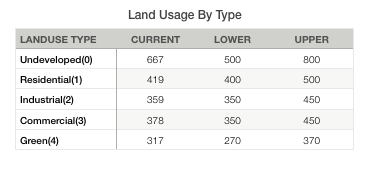
\includegraphics[width=4.in]{areas.png}
\caption{Synthetic Dataset used for initial evaluation}
\end{center}
\end{figure}

For attractiveness, each parcel is currently been assigned a random number from 0 to 1. \\

In the current approach we convert all the constraints also into objectives. So , now limits  for Landuse types would also come under the Objective function . We will later use constraint changed objectives only for filtering the results. So , our final output would consist of only results which follow the limit constraints.
We applied the algorithm  on the raster using the following objective functions. \\
\begin{itemize}
\item Contiguity
\item Attractiveness
\item Limit
\end{itemize}
\subsection{Results on Synthetic Dataset}
Following is the result of using NSGA on this dataset. As , we can compare with the original solution, the parent solution has lot of continuous groupings as compared to initial input/\\ 
\begin{figure}[h]
\begin{center}
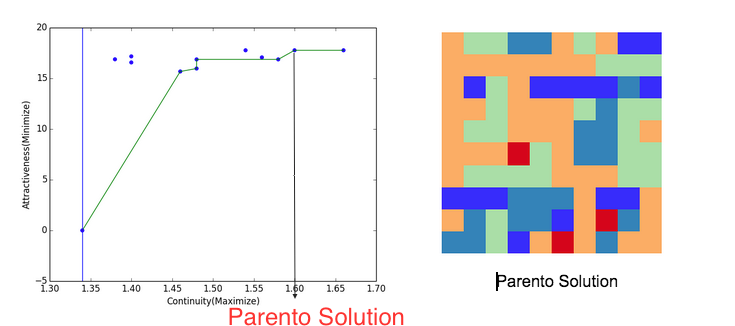
\includegraphics[width=3.5in]{res1.png}
\caption{NSGA Parento Solution}
\end{center}
\end{figure}

\paragraph{Single or Multi Objective encoding of Limits\\}

Here there are two approaches of using Limits as Objective. We can make Limit as a combined single objective or can have individual objectives corresponding to each LandUse type . \\
We ran the algorithm using the above objectives, where (X axis) we wanted to maximize continuity(compatibility) and wanted to minimize the attraction (Y axis) .\\

Here we can see the impact of taking limits as Single or Multi Objective Solution.
The results show the parent front (blue dots) formed where there is increase in contiguity (compatibility) of resulting solutions. The results are more compatible and still follow the limit constraints.(as can be seen from the continuity score). \\[.25cm]

The figure below shows the evaluation using NSGA. The  Limits are used as Objective, but its only used for filtering as limits are hard constraint. We only consider solutions which fall in the limits. \\
 One point to notice here is that (Figure 3), using limits as single objective gives similar results but multi objective gives too many other solutions too because if we have too many side objectives which we will eventually filter, then it will have an impact on our primary objectives.\\


\begin{figure}[h]
\begin{center}
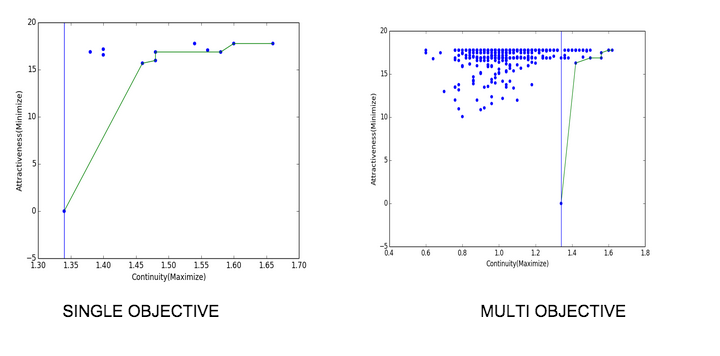
\includegraphics[width=4.in]{svd.png}
\caption{Using Limits as MultiObjective vs Single Objective}
\end{center}
\end{figure}

\section{North Carolina Dataset}

To validate our concepts on larger dataset, we took North Carolina Dataset, which consists of 43,000 parcels of varying size and 24 LandUse Types. Of these 43000, around 6000 parcels are allowed to be changed. Also, instead of attractiveness , we are provided suitability coefficient of each parcel, which basically describes its affinity to change. Along with the current allocation of lands type , we were also provided with manual drafted optimal solutions.(which we call A to E) . \\
\paragraph{Demand Constraints/Limits} The limit function(objective to minimize) is designed in such a way so as to minimize the constraint. Here we penalized the solution , which didn't follow the Limits. Also,  when it was with in the limits, we gave a negative cost, thus favoring this to fall with the limits. Problem with this V type of graph was it favored solution where limit is close to center and also was factored by the relative size of the particular LandType. We tried to get away with magnitude,by normalizing this factor by dividing by the difference of max and min.\\ Normalized Limits made sure that we didn't stayed within the limit and also not very high negative value is given to Landuse type which occupies the majority of the dataset.\\
\paragraph{Generate} We generated the initial dataset in the following way:
\begin{itemize}
\item Around 10 percent solutions were of type B, C, D, E .
\item We also took the initial configuration as the solution .
\item Rest were basically permutations of solutions of the optimal solutions, where each parcel had one out the values from A, B, C, D, E . Note that only these 6000 parcels are allowed to be changed , so changes are only possible for these parcels.
 \end{itemize}
In this implementation, we basically had Limits and Contiguity as Objective, so idea is to minimize Limits and increase the contiguity of the region. The entire dataset is represented as shown in the future below. \\
We did the analysis using first 
\begin{itemize} \item Contiguity and Limit 
\item  In the second case we took Contiguity, Limit and Attractiveness/Suitability.
\end{itemize}

\begin{figure}[h]
\begin{center}
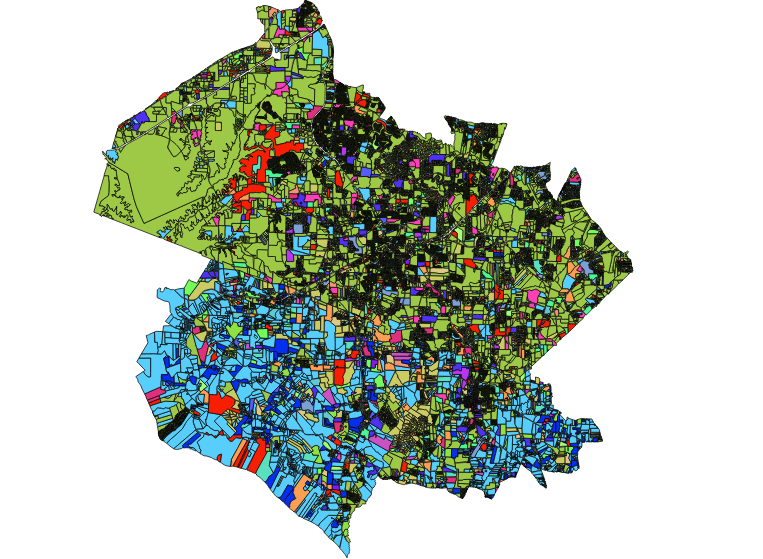
\includegraphics[width=4in]{nc.png}
\caption{North Carolina Dataset}
\end{center}
\end{figure}


\begin{figure}[h]
\begin{center}
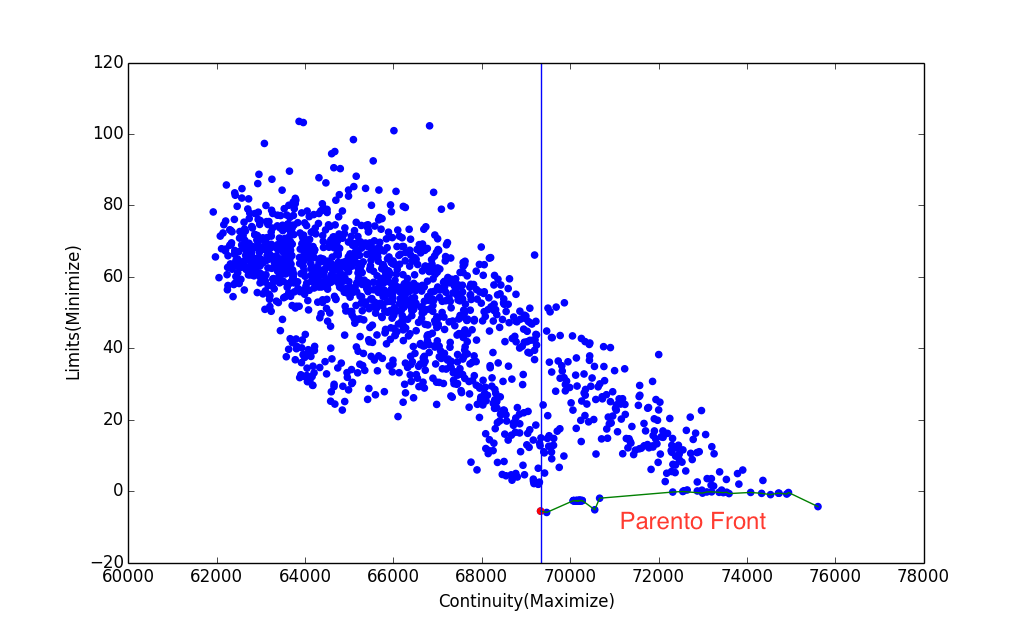
\includegraphics[width=3.5in]{Solutions.png}
\caption{Parento Front-Large Iterations}
\end{center}
\end{figure}
\begin{figure}[h]
\begin{center}
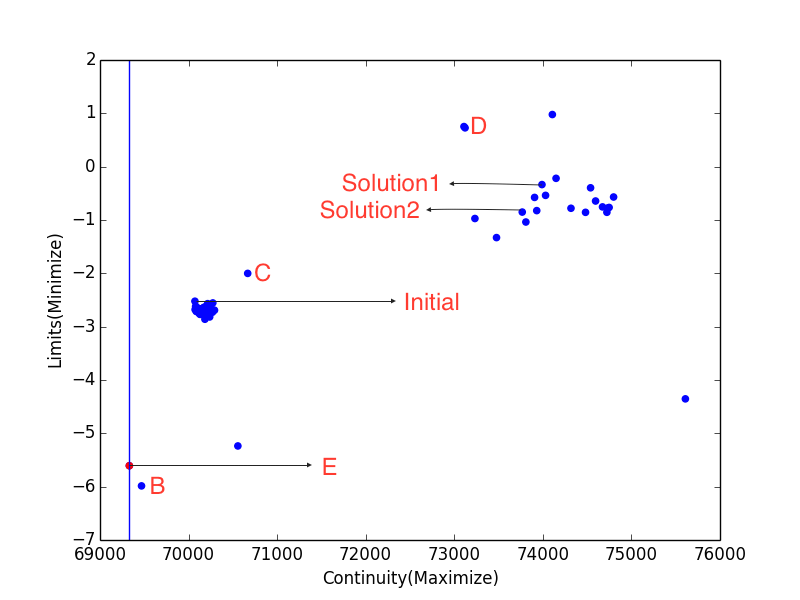
\includegraphics[width=3.5in]{ValidSolutions.png}
\caption{Valid Solutions -  Where Limit is satisfied for all the lands types}
\end{center}
\end{figure}


\begin{figure*}
\centering
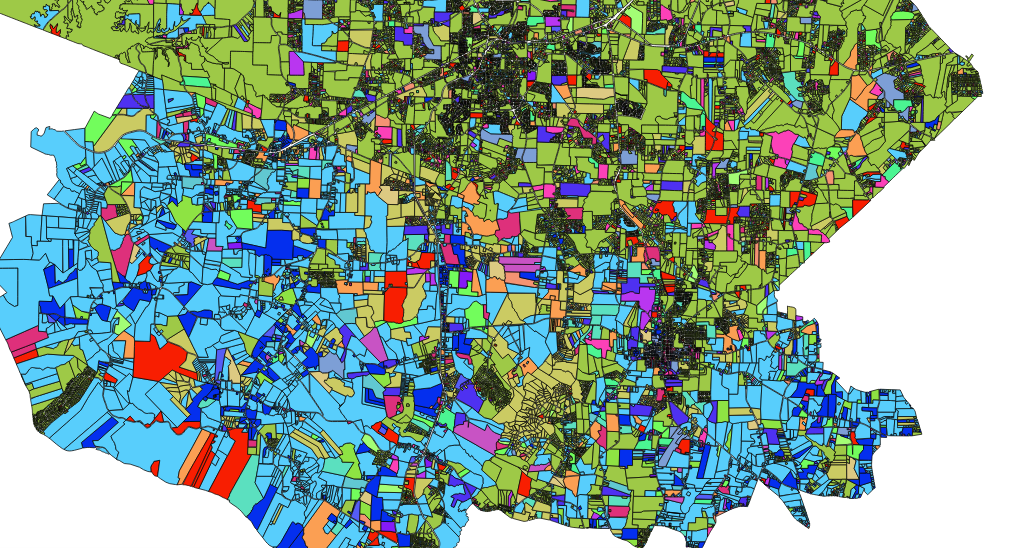
\includegraphics[width=4.5in]{Cont.png}
\caption{Initial}
\end{figure*}

\begin{figure*}
\centering
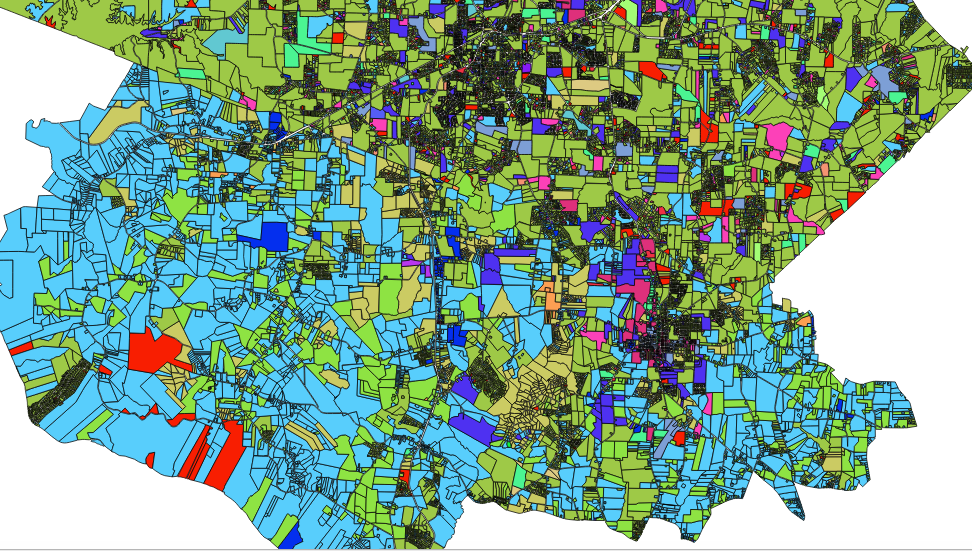
\includegraphics[width=4.5in]{ContSol1.png}
\caption{Solution-1 Contiguity-Limit}
\end{figure*}
\begin{figure*}
\centering
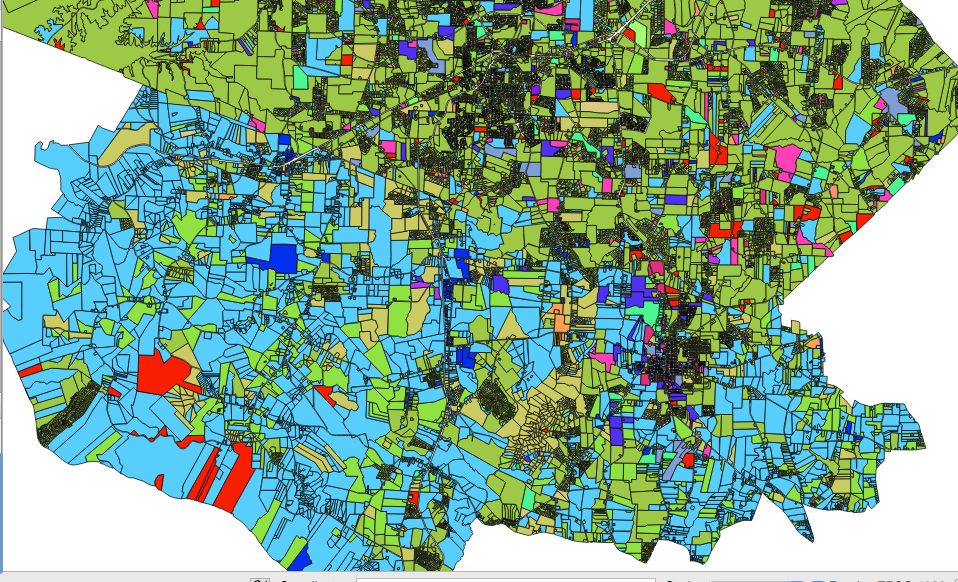
\includegraphics[width=4.5in]{ContSol2.png}
\caption{Solution - 2 Contiguity-Limit}
\end{figure*}


\subsubsection{Contiguity -Limit}
We ran the algorithm using the  initial generation as mentioned in earlier section :

After running NSGA , we got the following graph for Contiguity vs Limits.Figure 7 is output of 130 Population for 50 Generations . Thus, even in a small subset of cycles we can reach till the Parento Solutions. In Figure , E(manual) solution. Thus, it can be inferred that our solutions are better than and provides different alternates from the manual solutions in terms of Contiguity and Limit. We can clearly see that there was decrease in Limits as well as increase in Contiguity.\\
If we do closer evaluation between the current and the parent solution as shown in Figure 8-10, we can see that, there is more contiguity (central green part) in our solution compared original configuration, where we have cluster of many LandUseType. Also if we scrutinize further , we can see that many structures which were earlier separated by some margin are now joined. One more point to notice here is that using these two objectives , we basically saw some shifting and rearranging on parcels, as well as formation of contiguous of LandUse Types , which were initially present in small patches or were not at all present.  Now , in the next step, we add the suitability constraint, which will also force some changes depending upon the suitability value. \\
\subsubsection{Contiguity -Limit-Attractiveness}
Similarly , as in the last step, we ran NSGA but now using 3 objectives. We saw that in addition to solutions produced in earlier part, we also got solution, in which entire new allocation came to a region along with organization to increase contiguity.These solutions are also more continuous compared to the original state. This shows that attractiveness favors development of new LandUse Types in regions.\\

\begin{figure*}
\centering
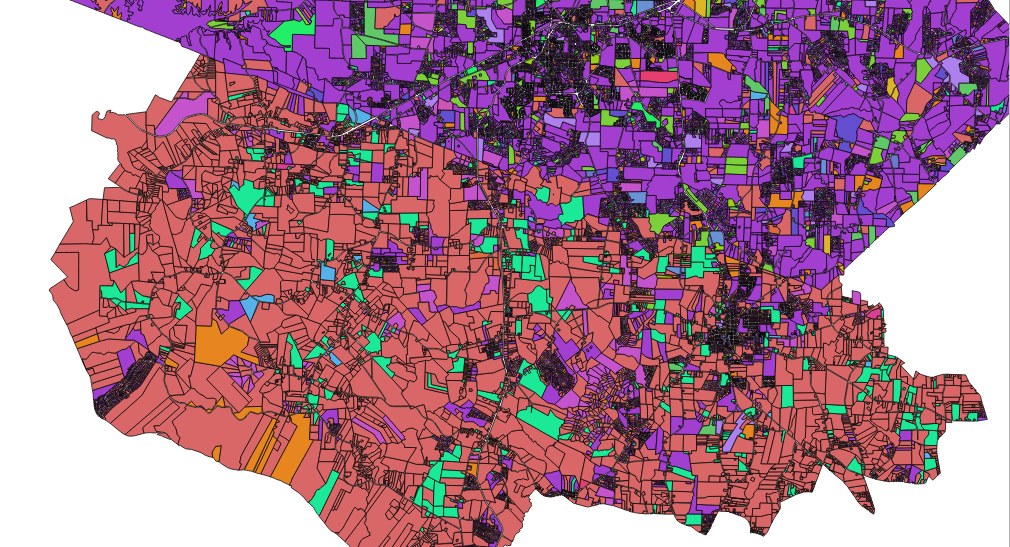
\includegraphics[width=4.5in]{orig1.png}
\caption{Initial - Using all 3 Objectives}
\end{figure*}

\begin{figure*}
\centering
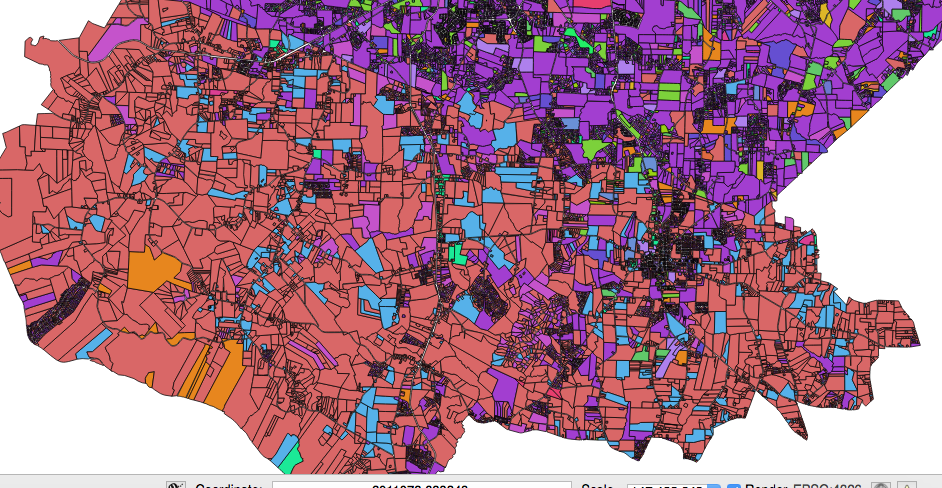
\includegraphics[width=4.5in]{Sol1.png}
\caption{Solution-1}
\end{figure*}
\begin{figure*}
\centering
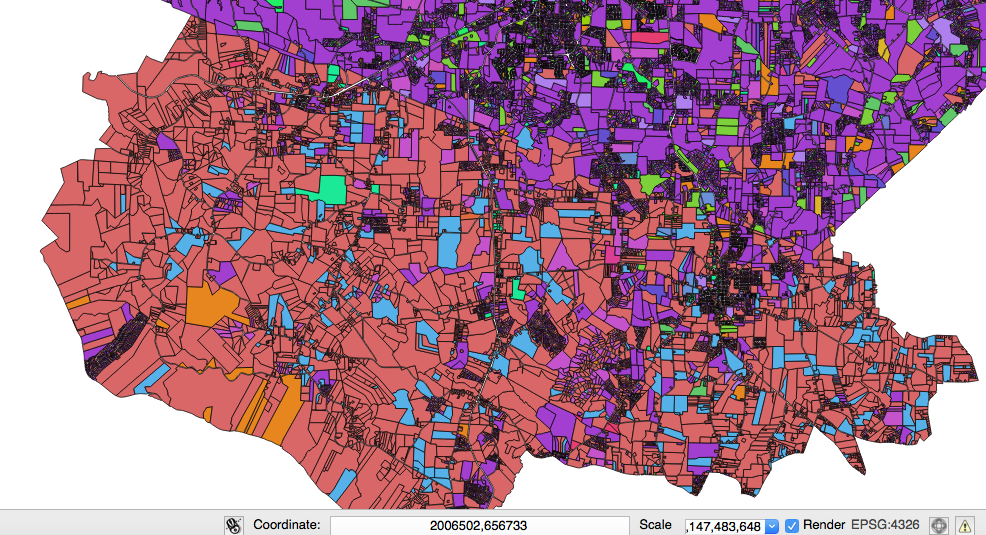
\includegraphics[width=4.5in]{Sol2.png}
\caption{Solution - 2}
\end{figure*}

 Thus, it shows that depending upon the requirement of a particular City/Area, we can come up with different solutions using NSGA by modifying the objective functions.
 
 \section{Discussion / Conclusion}
 In this problem, we were  used NSGA - II Algorithm on two datasets. First, in order to evaluate the Proposed Objective Equations we implemented these objectives on a small Synthetic dataset  and observed that by using genetic algorithms with the right set of Objective Equations, we can find various alternate solutions to City Planning problem. We defined a set of parameters which we used as input from the data and a set of variables which are expected to be evaluated. \\
 As Genetic Algorithm requires every thing in the form of objectives, so we had to convert all the constraints into objectives which we  later used only for filtering the results .  We used Limits here as objective which was later to to select solutions which followed the limit constraint rules for each of the LandUse Type. 
We implemented Continuity, Demand Constraint, Attractiveness and Suitability as Objectives and evaluated their impact on the dataset. We tried various approaches for Limits to best use it in an Objective Form. \\
We then implemented the same approach on North Carolina Dataset , where we were given some initial allocation along with some proposed solutions. Using this dataset , we were able to find solution , even better than those proposed in terms on contiguity and still satisfying  the Limit Constraint.\\

This project has various dimensions which can be continued in future research work. We had formed more linear equations, which would give even better results and at par which hand crafted ones if we can get information like some of the variables like road distance, distance to development etc. 
In algorithm, currently we span across the entire 43000 parcels, which make the search space wide. In future work, we can enhance this structure by doing NSGA only on the 6000 parcels that are allowed to be changed thus that would reduce the computation cost and would be able to get results from a smaller and a better search space. \\

Regarding the initial solutions , which we obtained  ( A to E) , they can also be automated using some search heuristics like Beam Search, A star , Numerical Programming on particular objectives. Combination os these along with some manual results can help in achieving even more realistic and better solutions.\\ 

 \appendix
\section{Summary of earlier work}

\subsubsection{Multi Objective Land Use Problem -Zielinska}

\paragraph*{Minimize Development of open space} Consider values Aj  for all cells that encode attractiveness for development for undeveloped cells. Idea is to set Aj very low for cells in open space. Add objective to minimise summation of (1-Aj) for all undeveloped cells that are developed. 
\paragraph*{Minimize redevelopment of urban areas}  Here idea is to avoid redevelopment of already developed areas . Here we define variable Rj as resistance for cell j to change from one developed form to another. This value will be high for compatible and contiguous neighbours and can be set low for cells which have low compatibility with his neighbours.
\paragraph*{Minimize incompatibilities between land use of site j and its neighbourhood } Here, there are 2 scenarios. First when an undeveloped cell is developed to type j. We want to minimize its compatibilities with its dominant neighbours. Thus , we would like to maximize developing cells with high compatibility. Second case is for  cells which are already developed and are changed from type i to j. Similar to previous premise , we want  to minimize its compatibilities with its dominant neighbours. 
\paragraph*{Minimizes the distance of new development to already developed sites } In order to increase compactness and avoid scattered developed areas , we want that newly developed areas should be in close proximity to the already developed areas.
\paragraph*{DBDC}
This step is important as it represents a contiguity and compactness constraint,which forces a user-specified neighbourhood infill development . It ensures that we will allocate to cell j if and only if the sum of the j?s initially and newly developed neighbours is at least equal to threshold b.\\[.25cm]


\subsubsection{Spatial multi-objective land use optimization: extensions to the  non- dominated sorting genetic algorithm-II -CAO}
\paragraph*{Minimizing land conversion costs}
Here it simply converts the minimization of conversion costs to the minimization of land use changes which clearly leads to greater economic benefits. However, this may rather lead towards to change from existing .

\paragraph*{Maximizing spatial accessibility}
Accessibility is important for land use planning not only because it reflects the operational efficiency of a city, but also because good accessibility planning can also improve social equity and lead to decreases in CO2 and related emissions which are largely generated inside the city from various human and automobile activities . The road system can be divided into three types:
roads that primarily serve residential neighborhoods, major routes for all transportation,
and routes that serve commercial and mixed uses.

Accessibility can be defined as how close or in proximity we have a Road of type R to location E[i,j].

Increasing land use compatibilities \\[.15cm]

The NSGA-II-MOLU model \\
Chromosome - Chromosome representation is a list or grid of genes, where the position of each
gene (cell) represents a unit and the land use of the unit is determined by its value.


\subsubsection*{Operators for NSGA-II-MOLU}
Paper on Cao was crucial from the perspective of defining operators to be used for NSGA II . \\
\paragraph*{Initialization operators}
In land use optimization problems, data pertaining to the existing land use status quo should be used as part of the iteration process, and then the initialization operators will create 90% random solutions and 10% land use status quo solutions as part of the initialized population. This initialization operator is called the problem-based initialization operator (PBIO).
\paragraph*{The crossover operator}
The crossover usually operates between the parents that are the two chromosomes from the population. However, in terms of the characteristics of the solution, self-reproduction might be made more efficient for each chromosome. The single parent crossover operator (XSP), which represents the two-dimensional structure of the spatial landscape, is applied to the land use optimization based on NSGA-II.

\paragraph*{Mutation operators}
There are two mutation operators. First operator(MPC) maintains diversity among solutions in a population, and the second is the mutation by constraint steering (MCS) which erases infeasible solutions from the population and enables the constraints to be met. 

\subsubsection{Evolutionary Multi-objective Optimization for landscape system design - Roberts}
 Based on Natural Habitats optimization . It uses methodology for generating estimates of the Pareto optimal set of designs for an evolving landscape in the rural urban fringe of a major metropolitan area.\\
 General landscape ecological principles
\begin{itemize}
  \item Patch size The term patch refers to a contiguous extent of natural features across
a landscape. In general, larger patches are better than smaller patches for
sustaining natural ecological functions.
  \item Number of patches Reducing the number of patches across a landscape reduces
the potential for recolonization and the potential for biodiversity by reducing the
availability of specific habitat types.
  \item Patch location If small patches are isolated islands then, depending on the
distance they are from other similar habitats, the populations they harbor are at a
greater or lesser risk of extinction.
  \item Patch shape -  Patches which are disc shaped allow for more interior habitat for a
given area and thus the potential for more interior species is increased. Convoluted
edges, i.e., lobes or peninsulas, encourage interactions with surroundings and favor
edge and/or generalist species.
\end{itemize}

\paragraph*{Objectives}
Considering the various features/concepts following are the objectives ,  the following four landscape level configuration patterns are deemed critical.

\begin{itemize}
  \item A few large patches of natural vegetation
 \item  Vegetated major stream or river corridors
 \item   Connectivity between larger patches with natural corridors and stepping stone patch configurations.
 \item  Heterogeneous patches of natural habitat dispersed throughout the landscape.
\end{itemize}
\paragraph*{Objective Functions}
\begin{itemize}
  \item OF1 - rewards maximizing the area of natural vegetation features in the entire data
set using the ELC classes normalized by total area.
 \item OF2 This objective rewards solutions with a few large patches of natural features which may be heterogeneous, e.g., comprising both woodland and wetland features.
 \item OF3 This objective favors connected structures of natural features across the landscape by maximizing the number of connected components in the top 1 to 5 (by area weighted, area?perimeter ratio) natural area subgraphs.
 \item OF4 This objective function rewards the formation of
discontinuous chains of smaller patches as pathways between larger vegetated
patches.
 \item OF5 This objective function rewards maximizing the area of agri/silvicultural features, normalized by total area,

\end{itemize}





\section{References}
Generated by bibtex from your ~.bib file.  Run latex,
then bibtex, then latex twice (to resolve references)
to create the ~.bbl file.  Insert that ~.bbl file into
the .tex source file and comment out
the command \texttt{{\char'134}thebibliography}.
% This next section command marks the start of
% Appendix B, and does not continue the present hierarchy
\section{More Help for the Hardy}
The sig-alternate.cls file itself is chock-full of succinct
and helpful comments.  If you consider yourself a moderately
experienced to expert user of \LaTeX, you may find reading
it useful but please remember not to change it.
%\balancecolumns % GM June 2007
% That's all folks!
\end{document}
